% Compact overview of the case's CD4AI feedback loop.
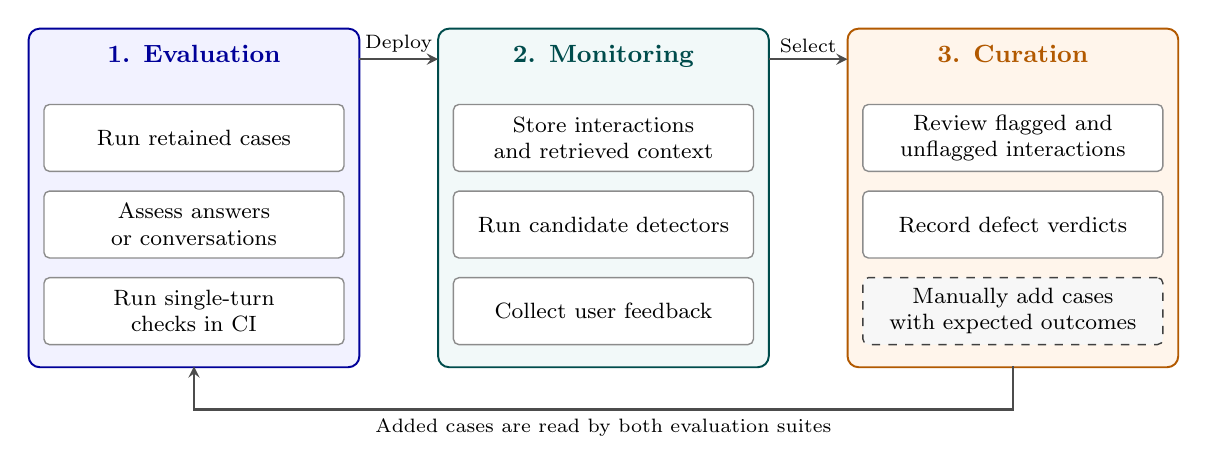
\begin{tikzpicture}[
  panel/.style={rounded corners=4pt, line width=0.7pt, minimum width=4.2cm,
    minimum height=4.3cm, anchor=north},
  head/.style={font=\small\bfseries, anchor=north, inner sep=0pt},
  sub/.style={font=\scriptsize\itshape, inner sep=0pt},
  item/.style={rounded corners=2pt, line width=0.5pt, draw=black!45, fill=white,
    text width=3.6cm, align=center, font=\footnotesize, inner sep=3pt,
    minimum height=0.85cm},
  team/.style={item, dashed, draw=black!75, fill=black!3},
  flow/.style={->, >=stealth, line width=0.8pt, draw=black!70},
  lbl/.style={font=\scriptsize, align=center, inner sep=1pt}
]
  \node[panel, draw=blue!60!black, fill=blue!5] at (0,0) {};
  \node[panel, draw=teal!60!black, fill=teal!5] at (5.2,0) {};
  \node[panel, draw=orange!70!black, fill=orange!8] at (10.4,0) {};
  \node[head, text=blue!60!black] at (0,-0.22) {1. Evaluation};
  \node[head, text=teal!60!black] at (5.2,-0.22) {2. Monitoring};
  \node[head, text=orange!70!black] at (10.4,-0.22) {3. Curation};
  \node[item] at (0,-1.4) {Run retained cases};
  \node[item] at (0,-2.5) {Assess answers\\or conversations};
  \node[item] at (0,-3.6) {Run single-turn\\checks in CI};
  \node[item] at (5.2,-1.4) {Store interactions\\and retrieved context};
  \node[item] at (5.2,-2.5) {Run candidate detectors};
  \node[item] at (5.2,-3.6) {Collect user feedback};
  \node[item] at (10.4,-1.4) {Review flagged and\\unflagged interactions};
  \node[item] at (10.4,-2.5) {Record defect verdicts};
  \node[team] at (10.4,-3.6) {Manually add cases\\with expected outcomes};

  \draw[flow] (2.1,-0.4) -- node[lbl, above=1pt] {Deploy} (3.1,-0.4);
  \draw[flow] (7.3,-0.4) -- node[lbl, above=1pt] {Select} (8.3,-0.4);
  \draw[flow] (10.4,-4.3) -- (10.4,-4.85) -- node[lbl, below=2pt]
    {Added cases are read by both evaluation suites} (0,-4.85) -- (0,-4.3);
\end{tikzpicture}
